\chapter{Conclusion}
\label{sec:final-conclusion}

As presented in the introduction, ESD are a major source of stress for electronic devices.
They can cause hardware failures, damaging permanently devices.
This class of issues has been studied for ten years, and is still the core of ESD research.
Recently, a new class of failures started to be considered.
Electrostatic discharges can cause temporary disturbances on devices.
In the context of always ever-more sensitive electronic devices and IC in particular, this is an issue.
Even more considering that electronic modules nowadays have increasingly large responsibilities in regard of our safety.
New trends for the autonomous car require electronic devices to take vital decisions for controlling the vehicule.
Guarantying safety of operation against electrostatic discharge is critical.

% Chap 1
A presentation of the context and topic is conducted in the introduction (chapter \ref{sec:global-intro}).
Chapter \ref{chap:1} is a review of the state of the art in ESD testing and soft-failure analysis.
It starts by describing common and recurrent test methods in the ESD field, and identifies relevant and realistic stress sources employed in laboratory environment.
A review of the literature on soft-failure analysis and prediction method is conducted afterward.
It showed that to this day there are rather few research on the topic of ESD-induced soft-failures at silicon level.
Many general-purpose observation techniques exist such as EMMI and near-field scan.
Among the simulation tools, it is common to find \gls{spice} simulation of course, and more advanced techniques such as 3D full-wave electromagnetic simulations or \gls{tcad} simulations.
These tools are highly interesting at the system and board level, to evaluate what fraction of an incoming discharge actually reach an integrated circuit.
It is important to notice that no solution exists so far to investigate at chip level how functions are disturbed by electrostatic discharges.
This point is a key part of the research presented in this document.

% Chap 2
In chapter \ref{chap:2}, a modeling method of electronic systems for ESD is detailed.
It relies and brings a few improvement over existing research conducted in the past on this topic.
A modular approach is employed, where each component is modeled individually to form a library, then assembled together in a hierarchical fashion.
Mostly physically based and most parameters can be extracted with simple tools, or by estimation where it is sometimes enough.
A concrete case study is presented with the modeling of a complex TLP generator.
It is perfect to illustrate a few key points for the modeling methods, and to demonstrate its accuracy against a lot of reference measurements.

% TLP-HMM
The development of this model and the insights gained in the process led to the development of a new pulse generator.
It reproduces the HMM waveform, one of the most widely used test pulse in the ESD field, but in a shielded and controlled environment.
The benefits are increased reproducibility of testing results and a flexibility for shaping the pulse waveform.
The prototype helped identified early issues and improvement to make.

% Correlation method
When comparing this generator to actual ESD guns and standard TLP, a new correlation method has been discovered.
It was validated successfully on 10 different ESD protections.
Correlation methods between ESD generators are extremely valuable because they can ultimately reduce testing time.
By testing a part with a single generator it is possible to predict the failure levels found with the others.
Before being able to do so, the correlation method should be tested on a much larger set of ESD protection.
Failure analysis on the destroyed parts should be conducted to verify if the failure mechanism remains identical between the different generator.

% Near-field current processing
In the last part of chapter \ref{chap:2}, a detailed post-processing method for on-chip near-field sensor has been presented.
It details the operation of the post-processing pipeline developed for this kind of sensor.
The processing script is released \cite{nfs-repository} under an open-source license to promote collaboration and future improvements on the topic.
Two different methods are evaluated and compared in order to reconstitute a current waveform from the voltage measured across the on-chip sensor.

% Chap 3
Chapter \ref{chap:3} presents a real case study where a complex analog function goes into restart because of an ESD.
The function is a primary regulator supply from a large automotive product.
It is put in a lowered \gls{bom} configuration where the external filtering is reduced to diminish the total application cost.
The ESD robustness of this configuration is studied, and a new failure is observed and explained.
After this analysis, it was decided to build a custom chip integrating this particular function, alongside with custom monitoring structures.
There were multiple objectives for making this test vehicle.
The first goal was to acquire waveforms inside the chip, using on-chip measurement structures and sensors, to validate that standard circuit simulations can be employed during an ESD event.
The second goal was to determine when and how analog function were disturbed by transient events, by using custom error detection cells.
This data was meant to validate the modelling methods presented later in the document (in chapter \ref{sec:methods-operating-esd-analysis}).
Creating an entire chip with custom cell designs and block reuse, alongside with the two application boards was extremely challenging.
This is especially true given limited resources and constraints inherent to the test vehicle process.
Despite extensive testing and validation, issues were met with the communication system responsible for outputting measurement data.
However, the two regulation functions and the on-chip sensors worked properly.
The extensive feedback and knowledge gained from the development of this custom chip is a ground work for new versions of this test vehicle and soft-failure research at silicon-level in general.
It should help define testchip architectures in the future, and with the appropriate fixes the communication system will constitute a reusable and convenient framework for interacting with on-chip monitoring systems.

% Chapter 4
Chapter \ref{sec:methods-operating-esd-analysis} is mainly focused on the development of tools for simulation environment.
The value of simulation tools is well known, because it enables to detect issues very early in the development cycle, which is extremely valuable for avoiding late issues and cutting the cost of fixing them late.
The main challenge for ESD at silicon-level is the complexity of the circuits and simulations.
Convergence issues are very common and sometimes extremely difficult to avoid.
The complexity of the circuits makes finding issues manually extremely hard.
Most of the time, it is required to manufacture a first silicon to test the parts against ESD and identify soft-failures.
To avoid those issues, new methods are required and two of them were proposed and explored during this research.

% First modelling method
The first method consist in characterizing and modeling some blocks of an analog function.
More specifically, the relationship between a given block input and block output.
Goal is to know at the silicon level what individual block was disturbed.
It is definitely a tool for the IC designers.
After a block model was constructed, it is possible to propagate from block to block a disturbance in the shape of a rectangular pulse of a given width and amplitude.
After each block, the disturbance changes, can increase or decrease in amplitude, become longer or shorter.
Ultimately, this method gives a "bounding box" of the disturbance on the final net, which is often sufficient to detect a functional failure.
This approach was tested with some success on the same case study than put previously on silicon.
It is still at its very early days, assumes a lot of simplifications and requires many improvements, however preliminary results tend to show it could actually be usable in a foreseeable future.
There are several challenges to overcome, in particular identifying the proper level in the hierarchy to model the blocks.
Also, the propagation path is considered unidirectional, the discharge propagates from an entry point to an outer point.
It is not really realistic, because it fact it spreads around the circuit.
However, it is important to make simplifications initially in order to get a prototype at work and evaluate what improvements or modifications are actually needed.

\begin{figure}[!h]
  \centering
  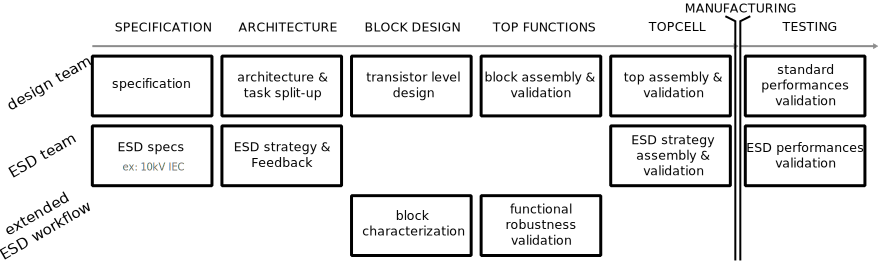
\includegraphics[width=\textwidth]{src/conclusion/figures/flow.pdf}
  \caption{IC conception flow and proposed improvements}
  \label{fig:new-flow}
\end{figure}

% Second modelling approach
The second modeling method is more focused on facilitating cooperation between IC manufacturers and equipment manufacturers.
It integrates well inside the SEED methodology, where interaction between these two actors helps design robust products against ESD with optimal cost and development time.
The objective is to characterize and model the relationship between an input pin and an output pin, and to check if a board simulation can be conducted with this black-box IC model.
It was shown that a TLP characterization constitutes a good base for a pin model, in particular for modeling inputs.
For output pins that are supposed to drive a potential in DC conditions, it was demonstrated that this method does not work and requires modifications.
The I(V) curve extracted with the TLP combined with a DC model fails to drive correctly the output voltage and current.
It is an interesting result that calls for more research on this topic.

% Proposal
% TODO Reduce and remove
Finally, a new method is proposed for IC design teams.
It is a complete proposal and has not been tested so far, however the concept seems highly promising with implications much further than ESD powered-on analysis and prediction.
The idea is to let analog designers define for their analog function blocks a set of assertions, or checks, that are mandatory for proper operation.
For instance, the check could be to ensure that a large enough voltage difference is present between the gate of a current mirror and ground.
It is also possible to add a check to ensure that a ground net never goes above a few hundred millivolts, otherwise it is either the sign that an ESD has induced a ground shift or that this net is simply floating.
Ultimately, each block could own its set of functional assertions, that would be checked by the simulator.
An appropriate tooling for observing the results and failed assertions is of course required, but it would be extremely helpful during power-on esd analysis to find which block was at fault, what block failed the first, understand how a disturbance has propagated inside the circuit and much more.
This tool could serve during the normal design flow, to guarantee functionality and immediately detect issues in block interconnections for instance.
There are no known technology locks that would present this method to be implemented.
Although not tested due to a lack of time, this tool is proposed and described inside this document because it was imagined from the experience gained with this research, and is believe to yield good and positive results.
Because of its modular nature (each block gets its own set of assertions), it fits extremely well inside the current IC design flow.
In particular, it is very friendly for modular IC design trends such as IP block reuse.
There are many challenges, in terms of user interaction, processing and display of results, integration with current simulation environments to be solved.
A first prototype could serve as a ground work to identify more accurately those challenges and prepare for a more advanced implementation.

% Final Conclusion
In conclusion, this work has explored many different topics and axes in the relatively new field of soft-failure ESD analysis.
The research could have been conducted in a very different manner.
For instance, it could have been a lot more IC-design-oriented.
A specific failure could have been studied extensively, a patch proposed and tested with a test-vehicle.
However, it was decided that this kind of highly specific highly focused approach would not be beneficial for future work.
Instead, more general methods and tools were explored.
At the end of this work, most of them remain merely at the prototyping phase.
We feel that this work provided new axes and research for future research, and that other people can actually takes those tools from a prototype to a production ready tool.
Improvements to near-field scan processing, improvements of the TLP-HMM and a larger validation of the TLP versus HMM correlation are probably the most simple follow-up work on the topic.
The bottom-up modeling method, the black-box IC method are still largely at the prototype phase and will require extensive research work before being production-ready.
Finally, the functional block checker, probably the most promising method among all those explored, needs initial work to make a prototype and evaluate the concept.
